\documentclass{beamer}

\usetheme{Madrid}
\usecolortheme{seahorse}
\useoutertheme[footline=authortitle]{miniframes}

\usepackage[utf8]{inputenc}
\usepackage{microtype}
\usepackage{graphicx}
\usepackage{booktabs}
\usepackage{subfig}

\usepackage{algorithm}
\usepackage[noend]{algpseudocode}

\newcommand{\en}[1]{\ifen#1\fi}
\newcommand{\sr}[1]{\ifsr#1\fi}

\algdef{SE}[SUBALG]{Indent}{EndIndent}{}{\algorithmicend\ }%
\algtext*{Indent}
\algtext*{EndIndent}

\en{\renewcommand{\algorithmicforall}{\textbf{for each}}}
\sr{\renewcommand{\algorithmicforall}{\textbf{za svaki}}}
\sr{\renewcommand{\algorithmicdo}{\textbf{:}}}
\sr{\renewcommand{\algorithmicif}{\textbf{ako je}}}
\sr{\renewcommand{\algorithmicthen}{\textbf{onda}}}

\title[Simple Merge Return Pass]{Simple Merge Return Pass}
\subtitle{\sr{Projekat u okviru kursa Konstrukcija kompilatora}\en{A Compiler Construction Course Project}}
\author{Konstantin Klima 476/2018}
\institute{\sr{Matematički fakultet, Univerzitet u Beogradu}\en{Faculty of Mathematics, University of Belgrade}}
\date{31.10.2025.}

\begin{document}

% Title slide
\begin{frame}
    \titlepage
\end{frame}

\begin{frame}
    \frametitle{\sr{Uvod}\en{Introduction}}
    \begin{itemize}
        \item \sr{\textit{mergereturn} - standardni LLVM optimizacijski pass }\en{\textit{mergereturn} - standard LLVM optimization pass}
        \item \sr{Spaja više return ili unreachable naredbi u jednu}\en{Merging multiple return points into one}
        \item \sr{Cilj je poboljšanje čitljivosti generisanog IR-a kao i daljih analiza i optimizacija}\en{Goal is to improve readability of generated IR code as well as further analyses and optimizations}

        \item \sr{Pripoznajemo tri slučaja koja treba obraditi:}\en{We recognize three cases to handle:}
        \begin {itemize}
            \item \sr{Više unreachable instrukcija - nastaju kao posledica exceptiona-a, instrukcija koje prekidaju tok izvršavanja ili prethodnih optimizacija}\en{Multiple unreachable instructions - they arise as a result of exceptions, instructions that interrupt the flow of execution}
            \item \sr{Više return instrukcija bez povratne vrednosti (void)}\en{Multiple return instructions with void return type}
            \item \sr{Više return instrukcija sa povratnom vrednošću različitom od void}\en{Multiple return instructions with non-void return type}
        \end{itemize}
    \end{itemize}
\end{frame}

% Algorithm slide
\begin{frame}
    \frametitle{\sr{Algoritam}\en{Algorithm}}
    \begin{algorithm}[H]
        \tiny
        \caption{Simple Merge Return Pass}
        \begin{algorithmic}
            \Indent
            \State $\textit{unrBlocks} \gets \text{\sr{niz blokova terminiranih unreachable instrukcijom}\en{array of blocks terminated by unreachable instruction}}$
            \State $\textit{retBlocks} \gets \text{\sr{niz blokova terminiranih return instrukcijom}\en{array of blocks terminated by return instruction}}$
            \EndIndent

            \State

            \ForAll{\sr{\textit{basicBlock} u funkciji \textit{F}}\en{\textit{basicBlock} in function \textit{F}}}
                \If{\sr{terminirajuća instrukcija za \textit{basicBlock} unreachable}\en{terminating instruction of \textit{basicBlock} is unreachable}}
                    \State \sr{dodaj \textit{basicBlock} u \textit{unrBlocks}}\en{Add \textit{basicBlock} to \textit{unrBlocks}}
                \EndIf

                \If{\sr{terminirajuća instrukcija za \textit{basicBlock} ret}\en{terminating instruction of \textit{basicBlock} is ret}}
                    \State \sr{dodaj \textit{basicBlock} u \textit{retBlocks}}\en{Add \textit{basicBlock} to \textit{retBlocks}}
                \EndIf
            \EndFor

            \State

            \If{$|\textit{unrBlocks}| > 1$}
                \State \sr{kreiraj novi blok \textit{unrBlock} sa unreachable instrukcijom}\en{create new block \textit{unrBlock} with Unreachable instruction}
                \ForAll{\sr{\textit{basicBlock} u \textit{unrBlocks}} \en{\textit{basicBlock} in \textit{unrBlocks}}}
                    \State \sr{zameni terminirajuću instrukciju u \textit{basicBlock} sa grananjem na \textit{unrBlock}}\en{replace terminating instruction in \textit{basicBlock} with branch to \textit{unrBlock}}
                \EndFor
            \EndIf

            \State

            \If{$|\textit{retBlocks}| > 1$}
                \State \sr{kreiraj novi blok \textit{retBlock} sa return instrukcijom}\en{create new block \textit{retBlock} with return instruction}
                \If{\sr{tip povratne vrednosti \textit{F} različit od void}\en{return type of \textit{F} is not void}}
                    \State \sr{kreiraj novu phi instrukciju}\en{create new phi instruction}
                    \State \sr{izmeni return instrukciju u \textit{retBlock} da učitava vrednost iz phi}\en{modify return instruction in \textit{retBlock} to load value from phi}
                \EndIf
                \ForAll{\sr{\textit{basicBlock} u \textit{retBlocks}} \en{\textit{basicBlock} in \textit{retBlocks}}}
                    \State \sr{zameni return instrukciju u \textit{basicBlock} sa grananjem na \textit{retBlock}}\en{replace return instruction in \textit{basicBlock} with branch to \textit{retBlock}}
                \EndFor
            \EndIf
        \end{algorithmic}
    \end{algorithm}
\end{frame}

\begin{frame}
    \frametitle{\sr{Napomene}\en{Notes}}
    \begin{itemize}
        \item \sr{Implementacija je testirana korišćenjem LLVM New Pass Managera - dodata je i legacy verzija koja zbog ograničenja lokalnog okruženja nije mogla da se testira.}\en{The implemented optimization was tested using the LLVM New Pass Manager - a legacy version was also added but could not be tested due to limitations of the local environment.}
        \item \sr{IR za primer sa višestrukim return instrukcijama je ručno izmenjen jer je frontend emitovao već optimizovan IR sa spojenim return instrukcijama (ovo nije bio slučaj kod unreachable primera)}\en{The IR for the example with multiple return instructions was manually modified because the frontend emitted already optimized IR with merged return instructions (this was not the case for unreachable examples)}
    \end{itemize}
\end{frame}

% First example slide - multiple unreachable instructions
\begin{frame}
    \frametitle{\sr{Primer 1: više Unreachable Instrukcija}\en{Example 1: Multiple Unreachable Instructions}}
    \begin{figure}
            \small
            \centering
            \subfloat[\centering \sr{Pre optimizacije}\en{Before optimization}]{{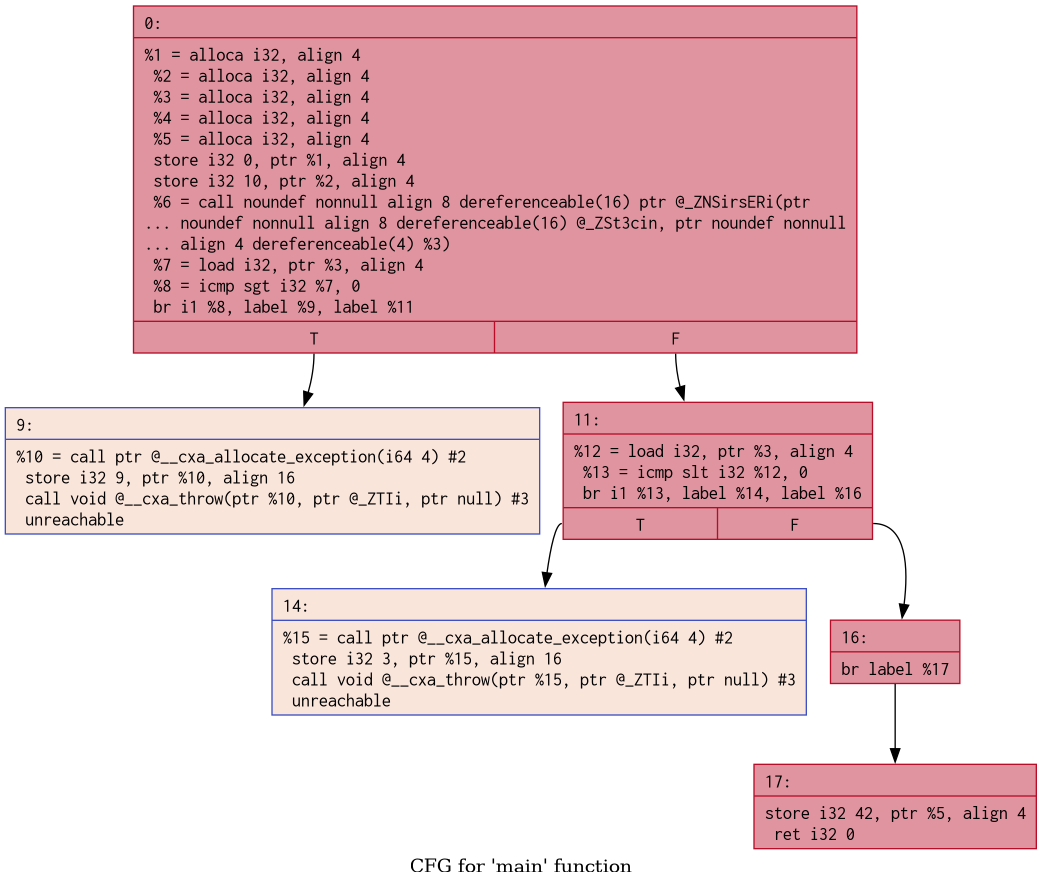
\includegraphics[width=5cm]{images/unreachable.png} }}%
            \qquad
            \subfloat[\centering \sr{Posle optimizacije}\en{After optimization}]{{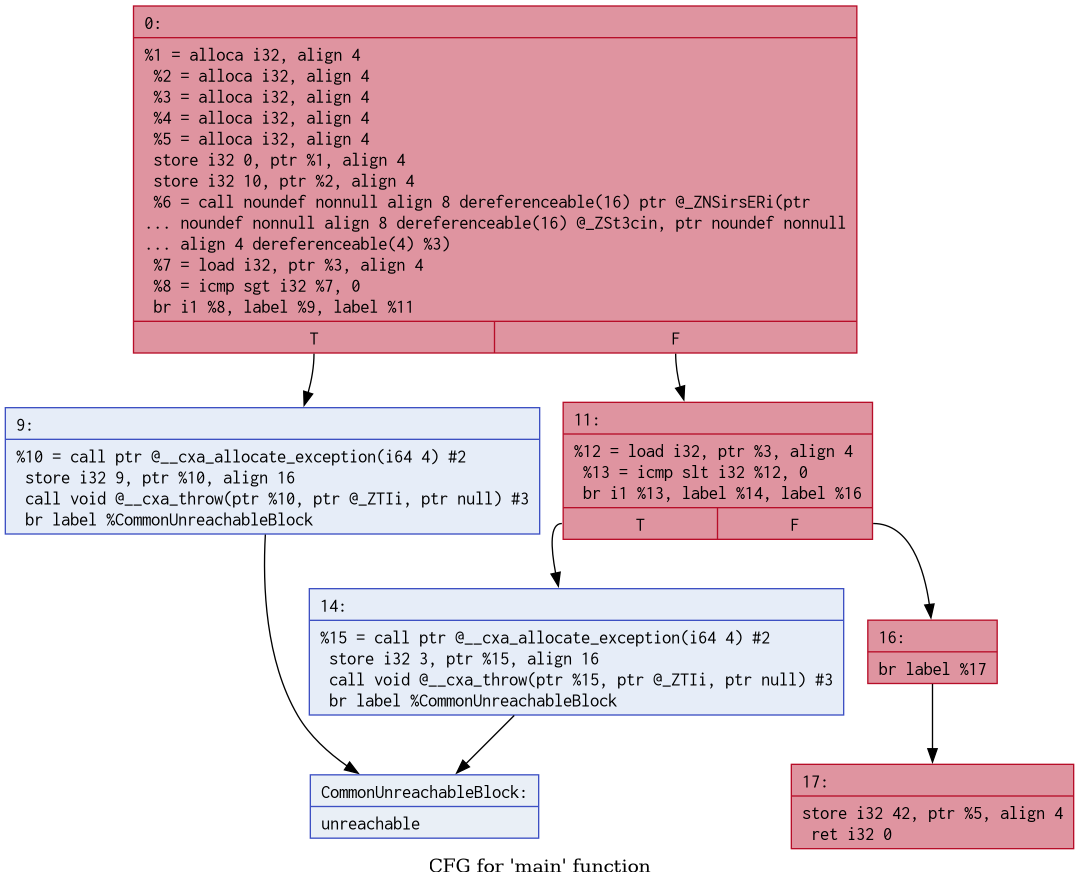
\includegraphics[width=5cm]{images/unreachable_optimized.png} }}%
    \end{figure}
\end{frame}

% Second example slide - multiple return instructions
\begin{frame}
    \frametitle{\sr{Primer 2: više Return Instrukcija}\en{Example 2: Multiple Return Instructions}}
    \begin{figure}
            \small
            \centering
            \subfloat[\centering \sr{Pre optimizacije}\en{Before optimization}]{{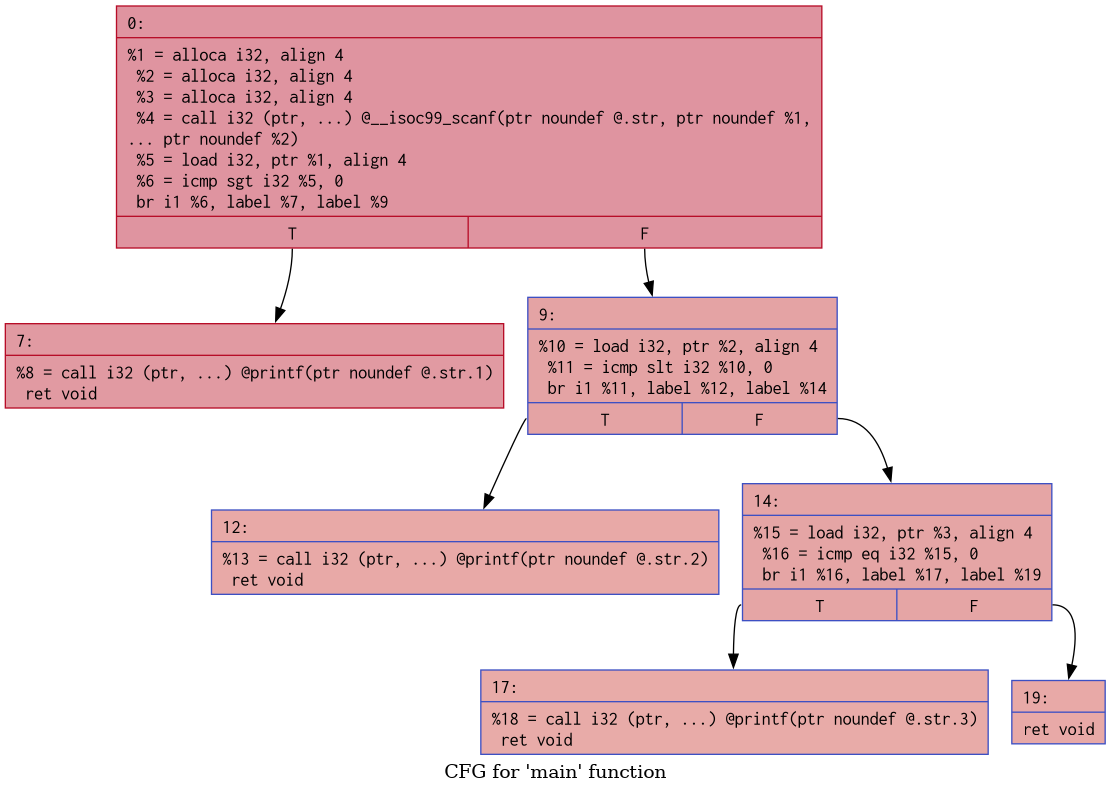
\includegraphics[width=5cm]{images/multiple_returns_void.png} }}%
            \qquad
            \subfloat[\centering \sr{Posle optimizacije}\en{After optimization}]{{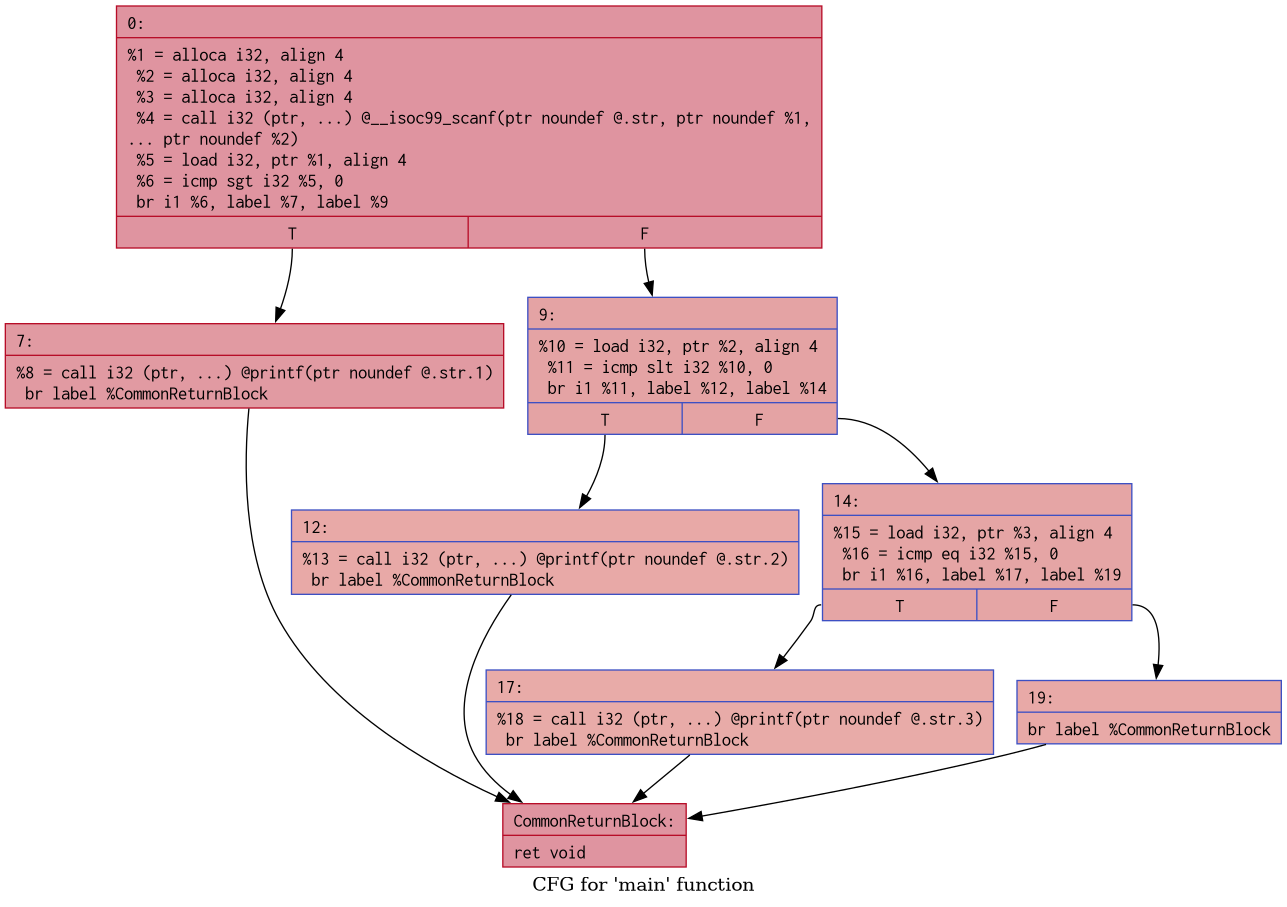
\includegraphics[width=5cm]{images/multiple_returns_void_optimized.png} }}%
    \end{figure}
\end{frame}

% Third example slide - multiple return instructions with non-void return type
\begin{frame}
    \frametitle{\sr{Primer 3: više Return Instrukcija sa povratnom vrednošću}\en{Example 3: Multiple Return Instructions with Non-Void Return Type}}
    \begin{figure}
            \small
            \centering
            \subfloat[\centering \sr{Pre optimizacije}\en{Before optimization}]{{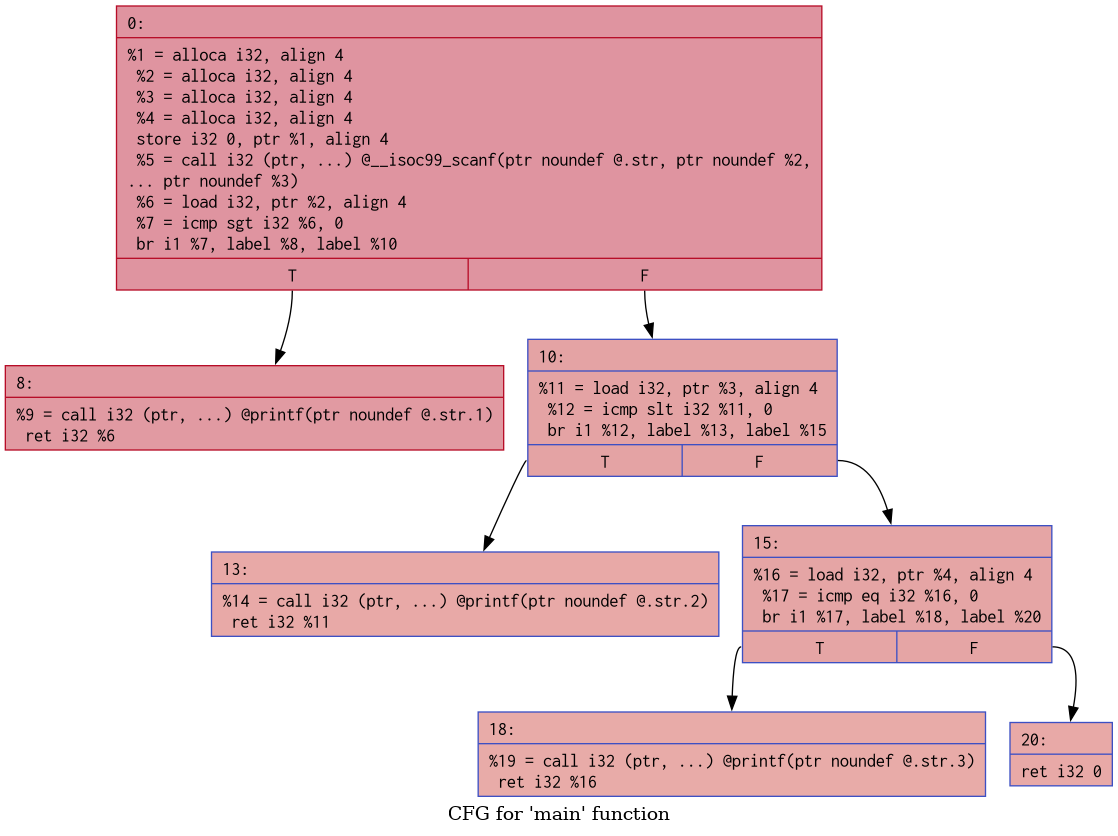
\includegraphics[width=5cm]{images/multiple_returns.png} }}%
            \qquad
            \subfloat[\centering \sr{Posle optimizacije}\en{After optimization}]{{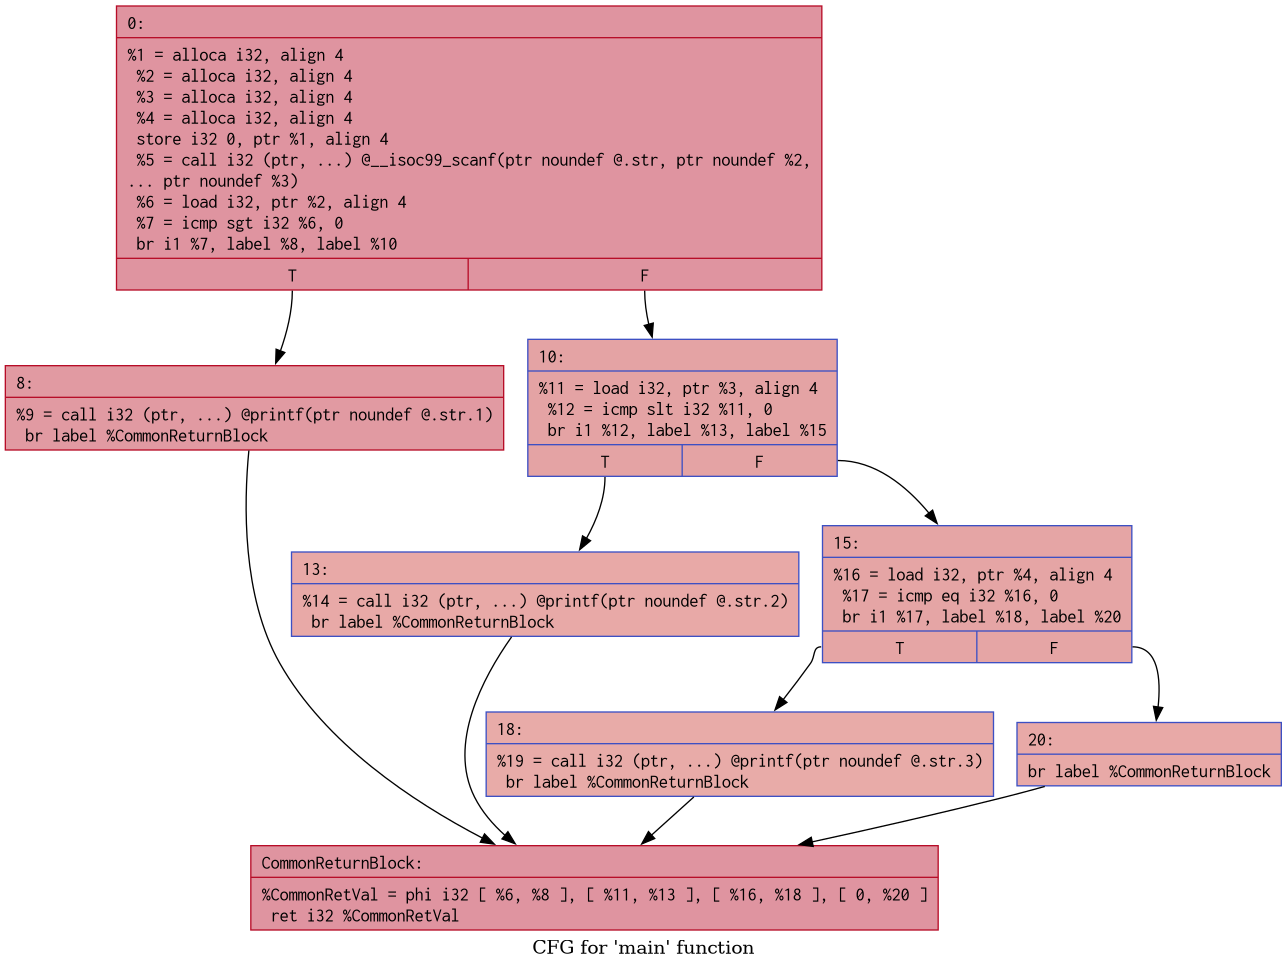
\includegraphics[width=5cm]{images/multiple_returns_optimized.png} }}%
    \end{figure}
\end{frame}

\begin{frame}
    \frametitle{\sr{Zaključak}\en{Conclusion}}
    \begin{itemize}
        \item \sr{Pri implementaciji neophodno je obratiti pažnju na različite tipove povratnih vrednosti i obezbediti da se propisno propagiraju pri zameni return instrukcija}\en{It is necessary to pay attention to different return types and ensure they are properly propagated when replacing return instructions}
        \item \sr{Optimizacija treba da obradi i unreachable instrukcije}\en{The optimization should also handle unreachable instructions}
        \item \sr{Kako ova optimizacija menja CFG, neophodno je ponoviti prethodno obavljene analize koje se oslanjaju na CFG}\en{Since this optimization changes the CFG, it is necessary to repeat previously performed analyses that rely on the CFG}
    \end{itemize}
\end{frame}

\end{document}